\section{Kapitel 1}

\subsection{Differentialgleichungen 1. Ordnung - Symbolische Lösungsverfahren}
\subsection{Gleichgewichtslösungen}
Die Gleichgewichtslösungen sind diejenigen Punkte, in welchen die Ableitung verschwindet:
\begin{equation*}
	\diffp{}{t}y(t) = 0
\end{equation*}
\subsection{Phasengerade und Integralkurven}
Bei der Phasengerade werden die Gleichgewichtslösungen in Funktion der Ableitung eingetragen. Dadurch kann die Stabilität eines Systems bestimmt werden. 

\subsection{Bifurkationen}
Gegeben ist eine autonome Differentialgleichung mit reellen Parametern.

\begin{equation*}
	\diffp{}{t}y(t) = f(a,y(t))
\end{equation*}

Suche die Gleichgewichtslösungen und unterscheide abhängig vom Parameter a in folgenden 3 Fällen:\\
\begin{itemize}
\item $a<0$
\item $a=0$
\item $a>0$
\end{itemize}
Für jeden dieser Fälle wird die Phasengerade gezeichnet und daraus kann man dann das entsprechende Bifurkationsdiagramm zeichnen. 

\begin{minipage}[h]{0.35\textwidth} 
	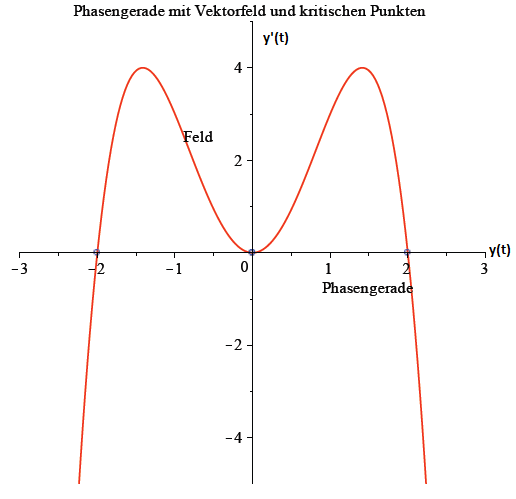
\includegraphics[width=1.0\textwidth]{images/Phasengerade.png}
\end{minipage}
\begin{minipage}[h]{0.35\textwidth}
	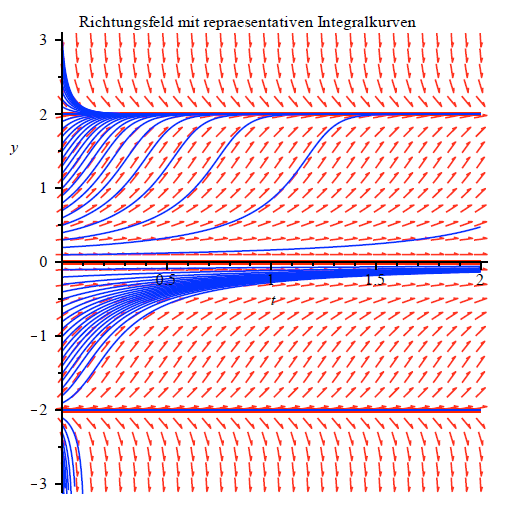
\includegraphics[width=1.0\textwidth]{images/Richtungsfeld.png}
\end{minipage}
\begin{tabular}{p{1.8cm}p{5cm}}
	$y(t) = -2$: & instabil \\
	$y(t) = 0$: & semistabil\\
	$y(t) = 2$: & asymtotisch stabil\\
\end{tabular}

\subsection{Bifurkationsdiagramm}
\begin{minipage}[h]{0.35\textwidth}
\[y'=y(a-y)\]
Kritische Punkte in Abhängikeit von $a$\\
\begin{tabbing}
Ausgezogen: \= Asymptotisch Stabil\\
Gestrichelt: \> Instabil\\
Zentrum: \> Semistabil\\
\end{tabbing}
\end{minipage}
\begin{minipage}[h]{0.35\textwidth}
	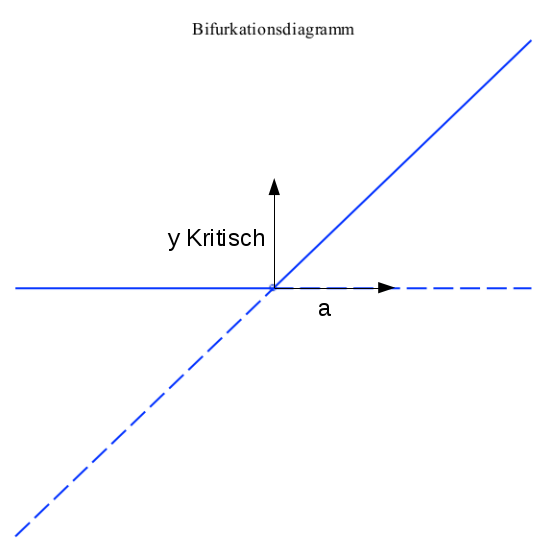
\includegraphics[width=1.0\textwidth]{images/Bifurkationsdiagramm.png}
\end{minipage}

\subsubsection{Allgemein 1. Ordnung}
\[ \dfrac{d}{dt}y(t)=f(t,y(t)) \qquad y(t_0)=y_0 \]
Eindeutige Lösung $\varphi(t)$ im Intervall falls $f(t,y(t))$ und $\dfrac{d \; f(t,y(t))}{dt}$ stetig im Intervall.